%%%%%%%%%%%%%%%%%%%%%%%%%%%%%%%%%%%%%%%%%
% Lachaise Assignment
% LaTeX Template
% Version 1.0 (26/6/2018)
%
% This template originates from:
% http://www.LaTeXTemplates.com
%
% Authors:
% Marion Lachaise & François Févotte
% Vel (vel@LaTeXTemplates.com)
%
% License:
% CC BY-NC-SA 3.0 (http://creativecommons.org/licenses/by-nc-sa/3.0/)
% 
%%%%%%%%%%%%%%%%%%%%%%%%%%%%%%%%%%%%%%%%%

%----------------------------------------------------------------------------------------
%	PACKAGES AND OTHER DOCUMENT CONFIGURATIONS
%----------------------------------------------------------------------------------------

\documentclass{article}
\usepackage{graphicx}
\usepackage{amsmath}
\usepackage{bm}
\usepackage{steinmetz}
\graphicspath{{images/}}
\usepackage{float} 
\usepackage{mathtools}
\usepackage[american,RPvoltages]{circuiTikz}
\usepackage{tikz, tikz-cd}
\usepackage{pgfplots}
\usepackage{siunitx}
\usetikzlibrary{spy,shapes,arrows, arrows.meta, bending}
\pgfplotsset{width=10cm,compat=1.18}
\input{structure.tex} % Include the file specifying the document structure and custom commands
\renewcommand{\figurename}{Figura}
\usepackage{tcolorbox}
\usepackage{lipsum}
\tcbuselibrary{listings,theorems,skins,vignette,raster,breakable,magazine,poster,fitting,hooks}
\usepackage{svg}
%----------------------------------------------------------------------------------------
%	ASSIGNMENT INFORMATION
%----------------------------------------------------------------------------------------

\title{Análisis senoidal en estado estable} % Title of the assignment
\author{Belmont Dubois} % Author name and email address

%----------------------------------------------------------------------------------------


\makeatletter
\pgfcircdeclarebipole{}{\ctikzvalof{bipoles/vsourcesin/height}}{sVpm}{\ctikzvalof{bipoles/vsourcesin/height}}{\ctikzvalof{bipoles/vsourcesin/width}}{
	
	\pgfsetlinewidth{\pgfkeysvalueof{/tikz/circuitikz/bipoles/thickness}\pgfstartlinewidth}
	\pgfpathellipse{\pgfpointorigin}{\pgfpoint{0}{\pgf@circ@res@up}}{\pgfpoint{\pgf@circ@res@left}{0}}
	\pgfusepath{draw}     
	\pgftext[bottom,rotate=90,y=\ctikzvalof{bipoles/vsourceam/margin}\pgf@circ@res@down]{\scriptsize$-$}
	\pgftext[top,rotate=90,y=\ctikzvalof{bipoles/vsourceam/margin}\pgf@circ@res@up]{\scriptsize$+$}
	
	\pgf@circ@res@up = .35\pgf@circ@res@up
	\pgfscope
	\pgftransformrotate{90}
	\pgfpathmoveto{\pgfpoint{-\pgf@circ@res@up}{0cm}}
	\pgfpathsine{\pgfpoint{.5\pgf@circ@res@up}{.4\pgf@circ@res@up}}
	\pgfpathcosine{\pgfpoint{.5\pgf@circ@res@up}{-.4\pgf@circ@res@up}}
	\pgfpathsine{\pgfpoint{.5\pgf@circ@res@up}{-.4\pgf@circ@res@up}}
	\pgfpathcosine{\pgfpoint{.5\pgf@circ@res@up}{.4\pgf@circ@res@up}}
	\pgfusepath{draw}
	\endpgfscope
}
\def\pgf@circ@sVpm@path#1{\pgf@circ@bipole@path{sVpm}{#1}}
\compattikzset{sinusoidal voltage source pm/.style = {\circuitikzbasekey, /tikz/to path=\pgf@circ@sVpm@path, \circuitikzbasekey/bipole/is voltage=true, \circuitikzbasekey/bipole/is voltageoutsideofsymbol=true, v=#1 }}
\compattikzset{sVpm/.style = {\comnpatname sinusoidal voltage source pm = #1}}

\pgfcircdeclarebipole{}{\ctikzvalof{bipoles/vsourcesin/height}}{sVpmh}{\ctikzvalof{bipoles/vsourcesin/height}}{\ctikzvalof{bipoles/vsourcesin/width}}{
	
	\pgfsetlinewidth{\pgfkeysvalueof{/tikz/circuitikz/bipoles/thickness}\pgfstartlinewidth}
	\pgfpathellipse{\pgfpointorigin}{\pgfpoint{0}{\pgf@circ@res@up}}{\pgfpoint{\pgf@circ@res@left}{0}}
	\pgfusepath{draw}     
	\pgftext[center,x=0.2\pgf@circ@res@down-\ctikzvalof{bipoles/vsourceam/margin}\pgf@circ@res@down]{\scriptsize$-$}
	\pgftext[top,rotate=90,y=\ctikzvalof{bipoles/vsourceam/margin}\pgf@circ@res@up]{\scriptsize$+$}
	
	\pgf@circ@res@up = .35\pgf@circ@res@up
	\pgfscope
	\pgftransformrotate{90}
	\pgfpathmoveto{\pgfpoint{-\pgf@circ@res@up}{0cm}}
	\pgfpathsine{\pgfpoint{.5\pgf@circ@res@up}{.4\pgf@circ@res@up}}
	\pgfpathcosine{\pgfpoint{.5\pgf@circ@res@up}{-.4\pgf@circ@res@up}}
	\pgfpathsine{\pgfpoint{.5\pgf@circ@res@up}{-.4\pgf@circ@res@up}}
	\pgfpathcosine{\pgfpoint{.5\pgf@circ@res@up}{.4\pgf@circ@res@up}}
	\pgfusepath{draw}
	\endpgfscope
}
\def\pgf@circ@sVpmh@path#1{\pgf@circ@bipole@path{sVpmh}{#1}}
\compattikzset{sinusoidal voltage source pmh/.style = {\circuitikzbasekey, /tikz/to path=\pgf@circ@sVpmh@path, \circuitikzbasekey/bipole/is voltage=true, \circuitikzbasekey/bipole/is voltageoutsideofsymbol=true, v=#1 }}
\compattikzset{sVpmh/.style = {\comnpatname sinusoidal voltage source pmh = #1}}
\makeatother

\begin{document}
	
	\maketitle % Print the title
	
	%----------------------------------------------------------------------------------------
	%	INTRODUCTION
	%----------------------------------------------------------------------------------------
	
	\section*{Circuitos de polarización prácticos para el BJT} % Unnumbered section
	Dado el circuito original de la figura \ref{fig:figura1} representado en el dominio del tiempo, nuestro primer paso es transformar el circuito al dominio fasorial o de frecuencia.
	% trim={<left> <lower> <right> <upper>}
	\begin{figure}[H]
		\centering
			\begin{circuitikz}[american, cute inductors,scale=0.9]
				\draw (0,0) to[sVpm, invert, l=$\begin{array}{c} v_s(t) \\ 12\cos{(1000 t + 45^{\circ}) V} \end{array}$] (0, 7)
					        to[R, l=$R_1$, a=4$\Omega$, -*] (4,7)
					        to[short, -*] (4,4)
					        to[R, l=$\begin{array}{c} R_2 \\ 20\Omega \end{array}$] (4,0)
					        to[short] (0,0);
				\draw (4,4) to[R, l=$R_3$, a=10$\Omega$, -*] (8,4)
					        to[L, l=$\begin{array}{c} L_1 \\ 5mH \end{array}$] (8,0)
					        to[short, -*] (4,0);
			    \draw (8,4) to[R, l=$R_5$, a=5$\Omega$] (12,4)
			    			to[C, l=$\begin{array}{c} C_1 \\ 100\mu F \end{array}$, f>_=$i_c(t)$] (12,0)
			    			to[short, -*] (8,0);
			    \draw (4,7) to[R, l=$R_4$, a=2$\Omega$] (12,7)
			    			to[short, -*] (12, 4);
			    \draw (4,0) to[short,-*] (6,0);
			    \draw (6,0) node[ground] {};
			\end{circuitikz}
		\caption{Circuito en el dominio del tiempo.}
		\label{fig:figura1}
	\end{figure}
	
	%\begin{figure}[H]
	%	\centering
	%	
\includegraphics[scale=1.5,trim={22.1cm 17.8cm 12.5cm 4.7cm},clip]{varios}
	%	\caption{Circuito en el dominio del tiempo}
	%	\label{fig:figura1}
	%\end{figure}
	
	\begin{align}
		12\cos (1000t + 45^{\circ}) \quad &\Longrightarrow \quad \nonumber 12\phase{45^{\circ}}, \quad \quad \omega = 1000 \,\,\, \text{rad}/s\\
		5mH \quad &\Longrightarrow \quad j\omega L = j(1000)(5\times10^{-3}) = j5 \Omega\nonumber\\ 
		100\mu F \quad &\Longrightarrow \quad \frac{1}{j\omega C} = \frac{1}{j(1000)(100\times10^{-6})} = -j10 \Omega  \nonumber
	\end{align}

	\noindent Así, el circuito equivalente en el dominio de la frecuencia es como se muestra en la figura \ref{fig:figura2}
	
	\begin{figure}[H]
		\centering
		\begin{circuitikz}[american, cute inductors,scale=0.9]
			\draw (0,0) to[sVpm, invert, l=$\begin{array}{c} \bm{V_s} \\ 12\phase{45^{\circ}} \, V \end{array}$] (0, 7)
			to[R, l=$R_1$, a=4$\Omega$, i=$\bm{I_1}$, -*] (4,7)
			to[short, -*] (4,4)
			to[R, l=$\begin{array}{c} R_2 \\ 20\Omega \end{array}$, i>_=$\bm{I_2}$] (4,0)
			to[short] (0,0);
			\draw (4,4) to[R, l=$R_3$, a=10$\Omega$, i>_=$\bm{I_3}$, -*] (8,4)
			to[L, l=$\begin{array}{c} L_1 \\ j5\Omega \end{array}$, i>_=$\bm{I_5}$] (8,0)
			to[short, -*] (4,0);
			\draw (8,4) to[R, l=$R_5$, a=5$\Omega$, i>_=$\bm{I_6}$] (12,4)
			to[C, l=$\begin{array}{c} C_1 \\ -j10\Omega \end{array}$, f>_=$\bm{I_c}$] (12,0)
			to[short, -*] (8,0);
			\draw (4,7) to[R, l=$R_4$, a=2$\Omega$, i>_=$\bm{I_4}$] (12,7)
			to[short, -*] (12, 4);
			\draw (4,0) to[short,-*] (6,0);
			\draw (6,0) node[ground] {};
			
			\draw (4,4) node[above left] {$\bm{V_A}$};
			\draw (8,4) node[above left] {$\bm{V_B}$};
			\draw (12,4) node[above left] {$\bm{V_C}$};
		\end{circuitikz}
		\caption{Circuito en el dominio de la frecuencia.}
		\label{fig:figura2}
	\end{figure}
	
	% trim={<left> <lower> <right> <upper>}
	%\begin{figure}[H]
	%	\centering
	%	
\includegraphics[scale=1.5,trim={22.4cm 12.5cm 12.6cm 10cm},clip]{varios}
	%	\caption{Circuito en el dominio de la frecuencia}
	%	\label{fig:figura2}
	%\end{figure}

	El análisis nodal se efectúa de la misma manera que el análisis de circuitos de cd, salvo que están implicados números complejos.
	Al aplicar la LCK en el nodo $V_A$ obtenemos
	\begin{align}
		\bm{I_1} = \bm{I_2} + \bm{I_3} + \bm{I_4}\nonumber
	\end{align}
	
	\noindent O bien
	\begin{align}
		\frac{\bm{V_S} - \bm{V_A}}{R_1} = \frac{\bm{V_A}}{R_2} + \frac{\bm{V_A} - \bm{V_B}}{R_3} + \frac{\bm{V_A} - \bm{V_C}}{R_4}\nonumber\\
		\frac{\bm{V_S} - \bm{V_A}}{4} = \frac{\bm{V_A}}{20} + \frac{\bm{V_A} - \bm{V_B}}{10} + \frac{\bm{V_A} - \bm{V_C}}{2}\nonumber\\
		5(\bm{V_S} - \bm{V_A}) = \bm{V_A} + 2(\bm{V_A} - \bm{V_B}) + 10(\bm{V_A} - \bm{V_C})\nonumber\\
		5\bm{V_S} - 5\bm{V_A} = \bm{V_A} + 2\bm{V_A} - 2\bm{V_B} + 10\bm{V_A} - 10\bm{V_C}\nonumber\\
		18\bm{V_A} - 2\bm{V_B} - 10\bm{V_C} = 5\bm{V_S}
	\end{align}

	\noindent Ahora aplicamos la LCK sobre el nodo $V_B$
	\begin{align}
		\bm{I_3} = \bm{I_5} + \bm{I_6}\nonumber 
	\end{align}
	\noindent O bien
	\begin{align}
		\frac{\bm{V_A} - \bm{V_B}}{R_3} = \frac{\bm{V_B}}{L_1} + \frac{\bm{V_B} - \bm{V_C}}{R_5}\nonumber\\
		\frac{\bm{V_A} - \bm{V_B}}{10} = \frac{\bm{V_B}}{j5} + \frac{\bm{V_B} - \bm{V_C}}{5}\nonumber\\
		\bm{V_A} - \bm{V_B} = -j2\bm{V_B} + 2(\bm{V_B} - \bm{V_C})\nonumber\\
		\bm{V_A} - \bm{V_B} = -j2\bm{V_B} + 2\bm{V_B} - 2\bm{V_C}\nonumber\\
		\bm{V_A} - (3 - j2)\bm{V_B} + 2\bm{V_C} = 0
	\end{align}

	\noindent Por último, empleamos la LCK en el nodo $V_C$
	\begin{align}
		\bm{I_4} + \bm{I_6} = \bm{I_C}\nonumber
	\end{align}
	\noindent Donde
	\begin{align}
		\frac{\bm{V_A} - \bm{V_C}}{R_4} + \frac{\bm{V_B} - \bm{V_C}}{R_5} = \frac{\bm{V_C}}{C_1}\nonumber\\
		\frac{\bm{V_A} - \bm{V_C}}{2} + \frac{\bm{V_B} - \bm{V_C}}{5} = -\frac{\bm{V_C}}{j10}\nonumber\\
		5(\bm{V_A} - \bm{V_C}) + 2(\bm{V_B} - \bm{V_C}) = j\bm{V_C}\nonumber\\
		5\bm{V_A} - 5\bm{V_C} + 2\bm{V_B} - 2\bm{V_C} -  j\bm{V_C} =0\nonumber\\
		5\bm{V_A} + 2\bm{V_B} - (7 + j)\bm{V_C} =0
	\end{align}

	\noindent Con lo cual tenemos el siguiente sistema de ecuaciones
	\begin{align}
		18\bm{V_A} - 2\bm{V_B} - 10\bm{V_C} &= 5\bm{V_S}\nonumber\\
		\bm{V_A} - (3 - j2)\bm{V_B} + 2\bm{V_C} &= 0\nonumber\\
		5\bm{V_A} + 2\bm{V_B} - (7 + j)\bm{V_C} &=0\nonumber
	\end{align}

	\noindent Donde 
	\[
		\Delta = \begin{vmatrix}
			18 & -2 & -10 \\
			1 & -(3-j2) & 2 \\
			5 & 2  &-(7+j)
		\end{vmatrix}
	\]
	
	\[
	\Delta_1 = \begin{vmatrix}
		-2 & -10 & 5\bm{V_S} \\
		-(3-j2) & 2 & 0 \\
		2  &-(7+j) & 0
	\end{vmatrix}
	\]
	
	\[
	\Delta_2 = \begin{vmatrix}
		18 & -10 & 5\bm{V_S} \\
		1 & 2 & 0 \\
		5 &-(7+j) & 0
	\end{vmatrix}
	\]
	
	\[
	\Delta_3 = \begin{vmatrix}
		18 & -2 & 5\bm{V_S} \\
		1 & -(3-j2) & 0 \\
		5 & 2  & 0
	\end{vmatrix}
	\]
	
	\noindent Nuestro objetivo es determinar el valor de la corriente $i_c(t)$, para esto nos enfocamos solamente en encontrar el voltaje en $V_c$, es decir
	
	\[
	\bm{V_C} = \frac{\Delta_3}{\Delta} =  \frac{\begin{vmatrix}
			18 & -2 & 5\bm{V_S} \\
			1 & -(3-j2) & 0 \\
			5 & 2  & 0
	\end{vmatrix}}{\begin{vmatrix}
	18 & -2 & -1 \\
	1 & -(3-j2) & 2 \\
	5 & 2  &-(7+j)
\end{vmatrix}} =  \frac{\begin{vmatrix}
18 & -2 & 5\bm{V_S} \\
1 & -(3-j2) & 0 \\
5 & 2  & 0\\
18 & -2 & 5\bm{V_S} \\
1 & -(3-j2) & 0
\end{vmatrix}}{\begin{vmatrix}
18 & -2 & -10 \\
1 & -(3-j2) & 2 \\
5 & 2  &-(7+j)\\
18 & -2 & -10 \\
1 & -(3-j2) & 2
\end{vmatrix}} = \frac{(85-j50)\bm{V_S}}{138-j100} = \frac{98.6154\phase{-30.4655^{\circ}}}{170.4230\phase{-35.9285^{\circ}}} \bm{V_S}
	\]
	
\begin{align}
	\bm{V_C} = 578.6503\times 10^{-3}\phase{5.4630^{\circ}}\bm{V_S}\nonumber
\end{align}

\noindent Donde $\bm{V_S} = 12\phase{45^{\circ}}$, por lo tanto

\begin{align}
	\bm{V_C} &= (578.6503\times 10^{-3}\phase{5.4630^{\circ}})(12\phase{45^{\circ}})\nonumber\\
	&= 6.9438\phase{50.4630^{\circ}} \,\, V\nonumber
\end{align}

\noindent Expresado en el dominio del tiempo, el voltaje en capacitor sería de:
\begin{align}
	v_c(t) = 6.9438\cos (1000t + 50.4630^{\circ}) \, V\nonumber
\end{align}

\noindent Una vez obtenido $V_C$ podemos determinar fácilmente la corriente por el capacitor
\begin{align}
	\bm{I_C} = \frac{\bm{V_C}}{-j10} =  \frac{6.9438\phase{50.4630^{\circ}}}{10\phase{-90	^{\circ}}} = 694.38 \times 10^{-3}\phase{140.4630^{\circ}} \,A \nonumber
\end{align}

\noindent Nuevamente, expresado en el dominio del tiempo, la corriente en el capacitor sería de:

\begin{tcolorbox}[colback=red!5!white,colframe=red!75!black,arc=0mm,boxrule=0mm,width=(\linewidth+0.5cm),extrude right by=-1.5cm]
	\begin{equation}
		i_c(t) =  694.38 \times 10^{-3} \cos (1000t + 140.4630^{\circ}) \nonumber
	\end{equation}
\end{tcolorbox}

\begin{figure}[H]
	\centering
	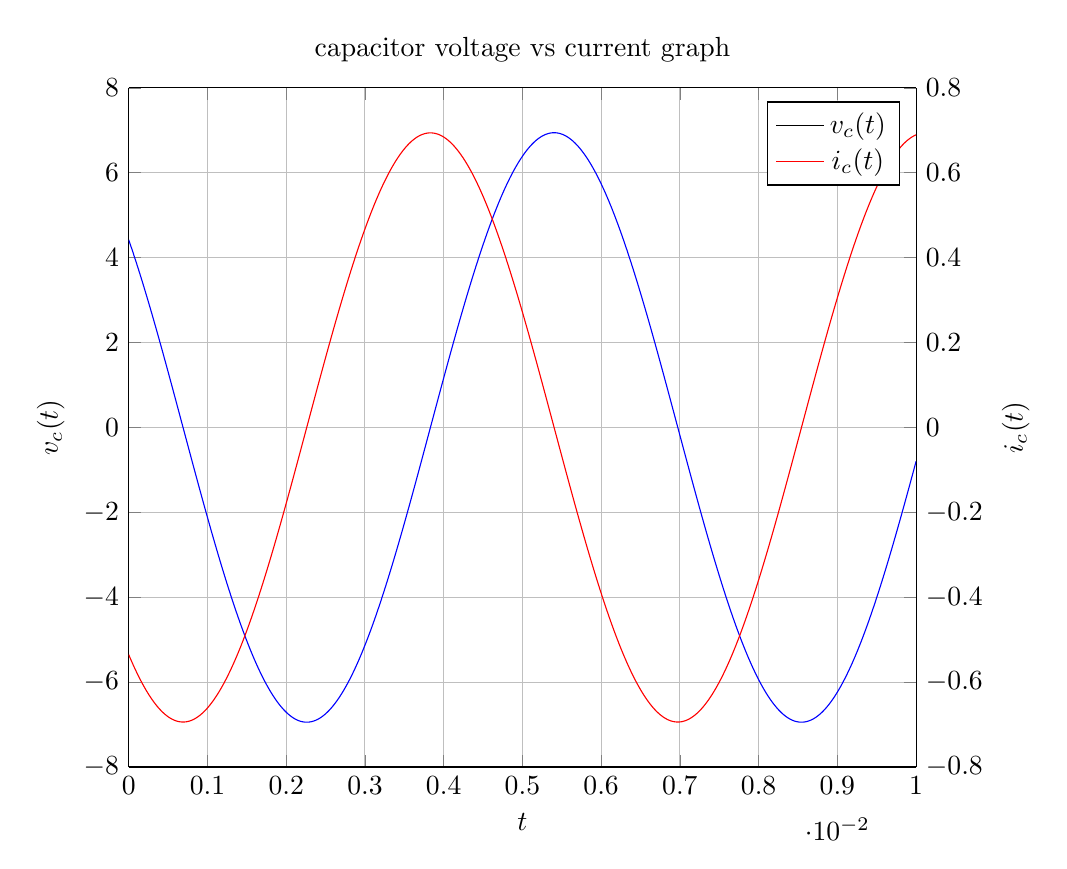
\begin{tikzpicture}
		% let both axes use the same layers
		\pgfplotsset{set layers}
		\begin{axis}[
			%legend entries={$x$},
			title= capacitor voltage vs current graph,
			scale only axis,
			xmin=0, xmax=0.01,
			ymin=-8,ymax=8,
			trig format plots=deg,
			domain=0:0.01,
			samples=1000,
			grid=major,
			axis y line*=left, % the '*' avoids arrow heads
			xlabel=$t$,
			ylabel=$v_c(t)$,
			restrict y to domain=-10:10
			]
			\addplot [blue] {6.9438*cos(1000*deg(x) + 50.4630)}; \label{plot_one}
			%\addlegendentry{$v_c(t)$}
			
		\end{axis}
		\begin{axis}[
			legend entries={$x_2$},
			scale only axis,
			xmin=0, xmax=0.01,
			ymin=-0.8,ymax=0.8,
			trig format plots=deg,
			domain=0:0.01,
			samples=1000,
			axis y line*=right,
			axis x line=none,
			ylabel=$i_c(t)$,
			restrict y to domain=-1:1
			]
			\addlegendimage{/pgfplots/refstyle=plot_one}\addlegendentry{$v_c(t)$}
			\addplot [red] {0.694*cos(1000*deg(x) + 140.4630)}; 
			\addlegendentry{$i_c(t)$}
			
		\end{axis}
	\end{tikzpicture}
\end{figure}

\begin{tikzpicture}
	\draw (2.5,0) node[npn] (t) {$Q_1$};
	\draw (0,0) to[C, l=$C_1$] (t.base); 
	\draw (t.base) node[above] {B};
	\draw (t.collector) node[left] {C};
	\draw (t.emitter) node[left] {E};
\end{tikzpicture}
 
\begin{figure}[H]
	\centering	
	\begin{tikzpicture}[]
		%\draw[step=1, gray,very thin] (-6.4,-6.4) grid (8.4,8.4);
		\draw[line width=0.5mm, fill=blue!10] (0,0) -- (0,6) -- (26.56:6.71) -- (0,0);
		\draw (2.5,3) to[cV, invert, l_=$A(v_2 - v_1)$] (2.5,1);
		\draw (2.5,1) node[ground] {};
		%\draw (8,3) node[above]{$v_o$} to[short, -o] (3,3);
		\draw (2.5,3) to[short, -o] (6.5,3) node[right]{$v_o$};
		%\draw (4,4) node[above left] {$\bm{V_A}$};
		%\draw[->]  (6,5) -- (7.5,3.1);
		\draw [blue!30,line width=0.5mm,-{Computer Modern Rightarrow[flex'=0.75]}]
		(7,4) .. controls (6.5,4) and (7,3.5) .. (6.5,3.2);
		\draw (7,4) node[blue!40,above right] {output};
		\draw (-2,5) node[above right]{$1$} to [short, f_={$i_1 = 0$}, o-o] (1,5) node[right]{$-$};
		\draw (-2,1) node[above right]{$2$} to [short, f_={$i_2 = 0$}, o-o] (1,1) node[right]{$+$};
		\draw [blue!30,line width=0.5mm,-{Computer Modern Rightarrow[flex'=0.75]}]
		(-1.5,6) .. controls (-1.6,5.5) and (-1.3,5.3) .. (-1.6,5.1);
		\draw (-1.5,6) node[blue!40,above] {Inverting input};
		\draw [blue!30,line width=0.5mm,-{Computer Modern Rightarrow[flex'=0.75]}]
		(-1,0) .. controls (-2,0.3) and (-2,0.6) .. (-2,0.9);
		\draw (-1,-0.2) node[blue!40,below] {Noninverting input};
		\draw (-3,5) to[short, -o] (-2,5);
		\draw (-3,5) to[V, invert, l_=$v_1$] (-3,3);
		\draw (-3,3) node[ground] {};
		\draw (-3,1) to[short,-o] (-2,1);
		\draw (-3,1) to[V, invert, l_=$v_2$] (-3,-1);
		\draw (-3,-1) node[ground] {};
	\end{tikzpicture}
	\caption{Circuito equivalente del amplificador operacional ideal.}	
\end{figure} 


\end{document}


